\subsection{Molecular vibration}
\label{sec:mol-vibration}

A simple ball and spring harmonic oscillator model from classical mechanics can explain molecular vibrations. However, principles from quantum mechanics are required to describe vibrational energy levels and transitions between them.

Atoms are the basic unit of molecules, and covalent bonds hold them together. The distance between atoms or the length of chemical bonds is not fixed. Therefore, molecules can vibrate when excited to a higher energy state by absorbing a resonant photon of electromagnetic radiation in the infrared region.
\begin{figure}[!htb]
    \centering
    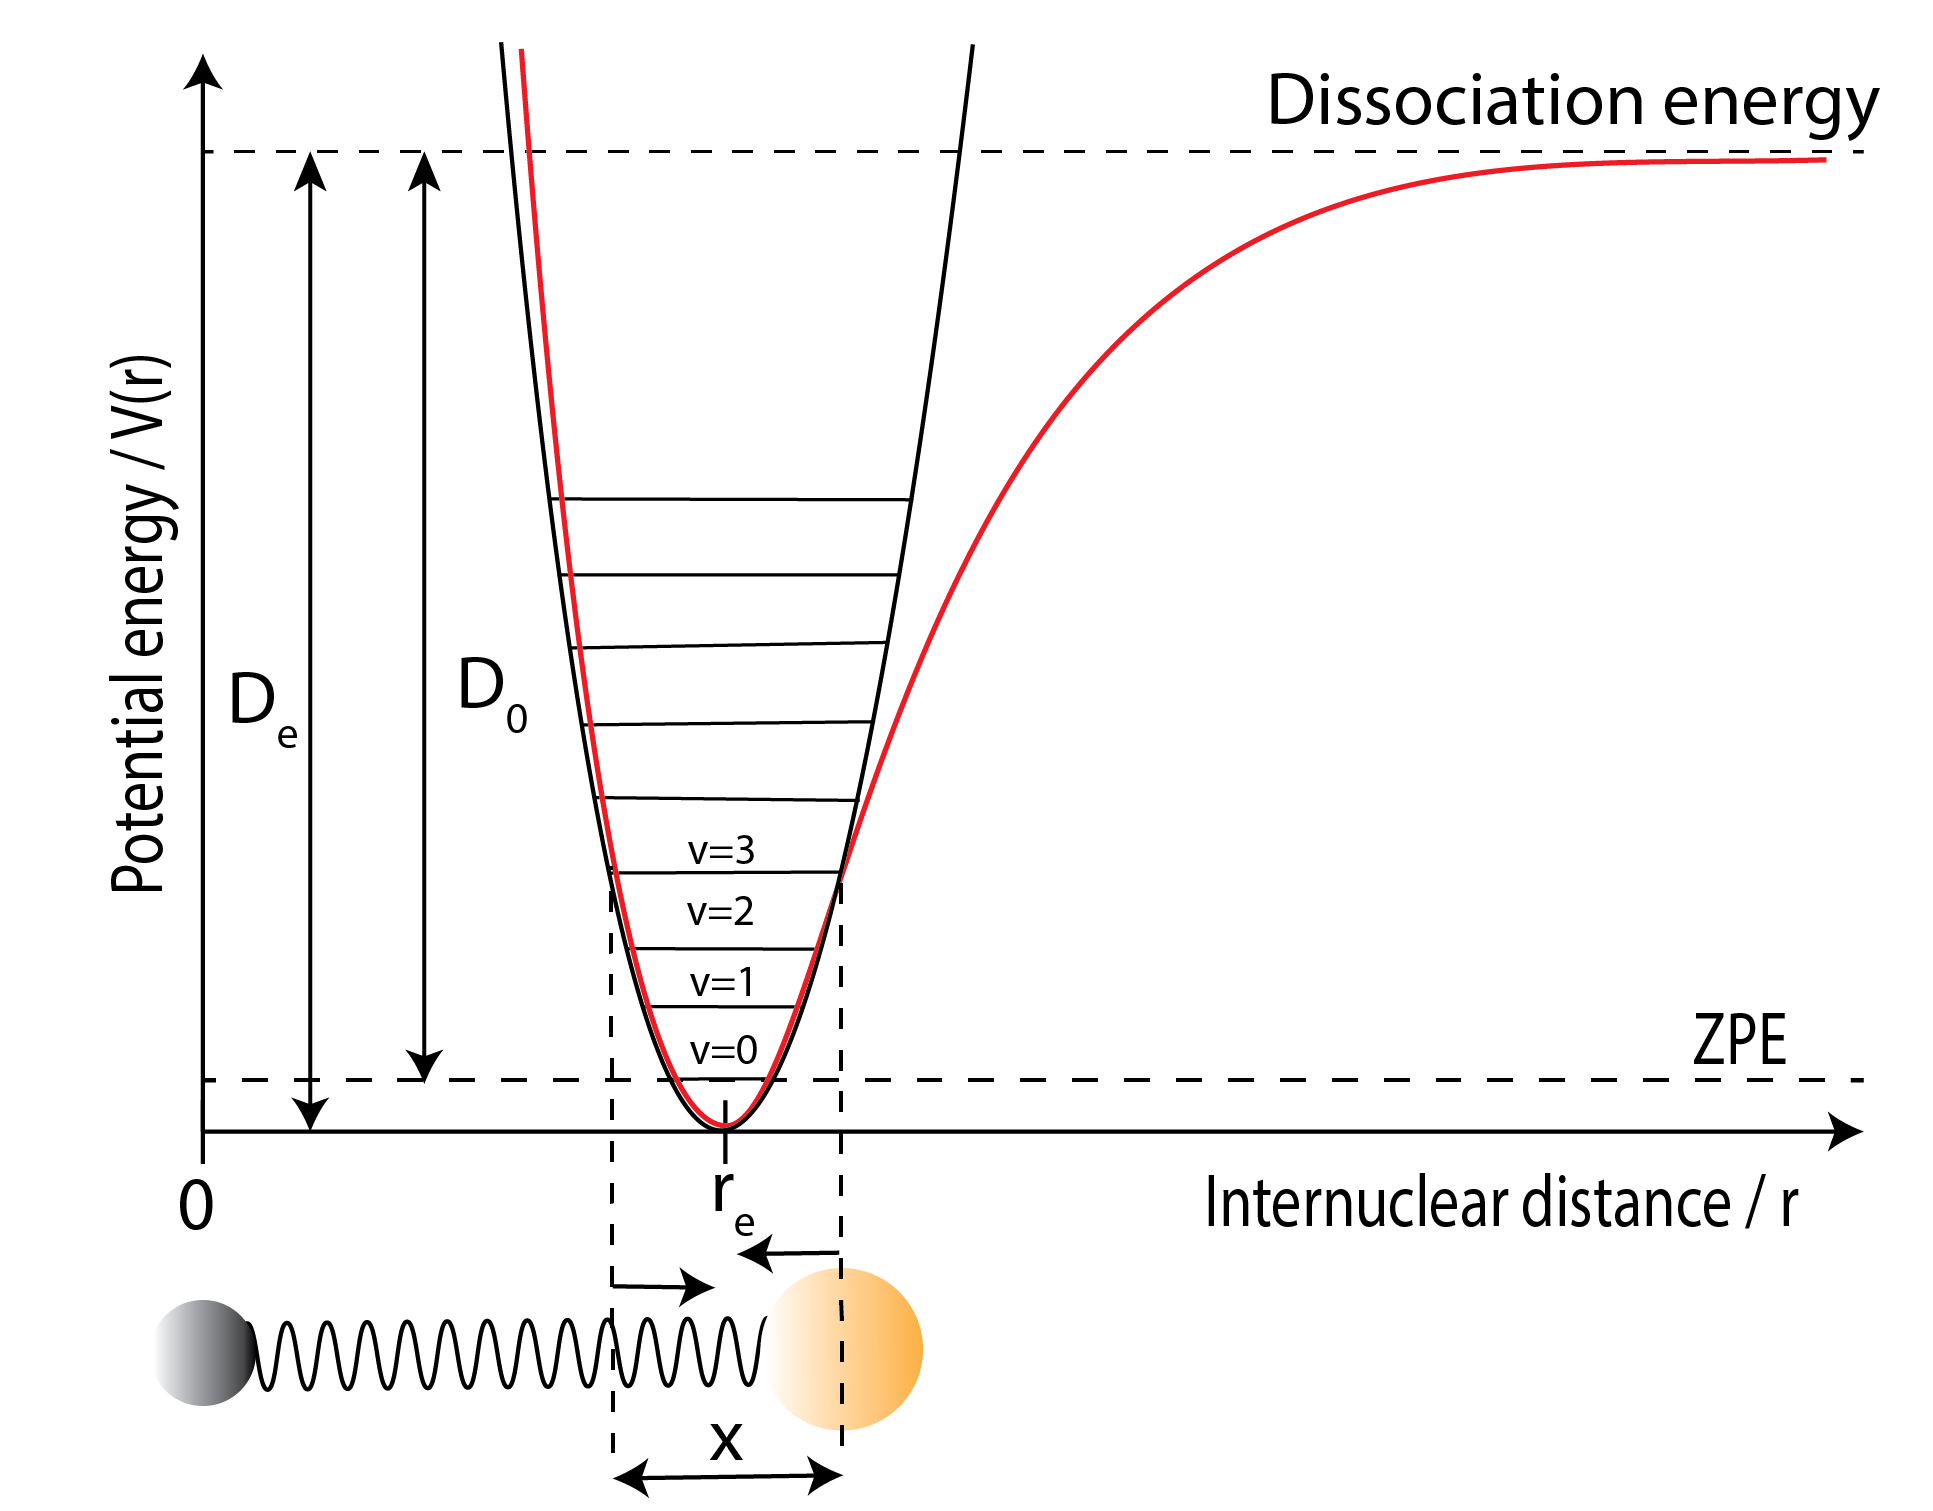
\includegraphics[scale=0.5]{figures/methods/harmonic-oscillator-01.png}
    \caption{Heteronuclear diatomic molecule (solid circles at the bottom) vibrating at energy level $v=3$. The black and red curve represent harmonic and anharmonic (Morse) potential energy curves, respectively. $r_e$ is the equilibrium bond length, $D_0$ and $D_e$ correspond to dissociation energy with and without ZPE (zero-point energy) correction, respectively. }
    \label{fig:vibration:oscillator}
\end{figure}

\subsubsection{Diatomic molecules}
\label{sec:mol-vibration:diatomic}

Assuming a simple ball and spring harmonic oscillator model as shown in Figure \ref{fig:vibration:oscillator} gives us the potential energy ($V$) from Hooke's law:
\[\text{Restoring force} = - \frac{dV(x)}{dx} = -kx\]
where $x=r-r_e$ and $k$ is force constant:

\begin{equation}
    \label{eqn:harmonic-oscillator:V(x)}
    V(x) = \frac{1}{2} k x^2
\end{equation}

Substituting, equation \ref{eqn:harmonic-oscillator:V(x)} in equations \ref{eqn:quantum:Hamiltonian} and \ref{eqn:quantum:wave-eqn}, we get the Schr\"odinger equation for 1D-oscillator:

\begin{equation}
    \label{eqn:hamiltonian-harmonic:V(x)}
    \left( -\frac{\hbar^2}{2\mu} \frac{d}{d x^2} + \frac{1}{2} k x^2 \right ) \psi_v(x) = E_v\psi_v(x)
\end{equation}
where $\mu$ is the reduced mass.

Equation \ref{eqn:hamiltonian-harmonic:V(x)} can be solved to obtain $E_v$ as given below:

\begin{equation}
    \label{eqn:vibrational-energy-Ev}
    E_v = \left( v + \frac{1}{2} \right) h \text{v} = \left( v + \frac{1}{2} \right) hc\omega
\end{equation}

where v is classical vibrational frequency, $\text{v}=\frac{1}{2\pi}\enclose{\frac{k}{\mu}}^{1/2}$, $\omega$ is vibrational wavenumber, the vibrational quantum number is $v=0, 1, 2, ...$ .


Equation \ref{eqn:vibrational-energy-Ev} shows that under the harmonic approximation, the vibrational quantum levels are equally spaced by $\hbar\omega$ and the Zero-point energy (ZPE) i.e., $E_v(v=0)=\frac{1}{2}\hbar\omega$. As shown in Figure \ref{fig:vibration:oscillator}, the ZPE is the minimum energy the molecule may have even at absolute zero temperature because of the uncertainty principle.

The energy terms are usually referred to in wavenumbers [\wn], so we can write Eq. \ref{eqn:vibrational-energy-Ev} as:

\begin{equation}
    \label{eqn:Ev-Gv}
    \frac{E_v}{hc} = \omega \enclose{v + \frac{1}{2}} = G(v)
\end{equation}

where $G(v)$ is the vibrational term value in dimensions of wavenumber, \wn.

As shown in Figure \ref{fig:vibration:oscillator}, the Morse $V(r)$ curve, the actual diatomic molecule is not accurately harmonics, especially when $r \gg r_e$. To account for anharmonicity, the harmonic oscillator term value are modified to a power series in $\enclose{v + \frac{1}{2}}$:

\[G(v) = \omega_e \enclose{v + \frac{1}{2}} - \omega_e x_e \enclose{v + \frac{1}{2}}^2 + \omega_e y_e \enclose{v + \frac{1}{2}}^3 + ...\]

where $\omega_e$ is the vibration wavenumber that a classical oscillator would have for an infinitesimal displacement from equilibrium. $\omega_e x_e$, $\omega_e y_e$, ... are the anharmonic constants.

To determine, say $\omega_e$ and $\omega_e x_e$, at least two transition wavenumbers must be obtained such as $G(1)-G(0)=\omega_0$ and $G(2)-G(1)=\omega_1$. The dissociation energy $D_e$ is given approximately (since including only $\omega_e x_e$ anharmonic term) by:
\[D_e \simeq \frac{\omega_e^2}{4\omega_e x_e}\]\\

\subsubsection{Polyatomic molecules}
\label{sec:mol-vibration:polyatomic}
The vibrational modes of an  $N$-atomic molecule are give by $3N-5$ and $3N-6$ normal vibration modes for linear and non-linear configuration, respectively.

Polyatomic vibrational modes are much more complicated to treat theoretically than diatomic. As shown in Figure \ref{fig:oscillator:water}, a simple ball-spring model with 3-atoms (H$_2$O), even if one of the nuclei is given a sudden displacement, the whole system undergoes very complicated vibrational motions (bending and stretching); this is known as Lissajous motion. For H$_2$O, we get $3(3)-6=3$ normal modes of vibrations ($v_1-v_3$). In general, a normal vibration mode is one in which all the nuclei undergo in-phase harmonic motion with the same frequency but typically with different amplitude.
\begin{figure}[!htb]
    \centering
    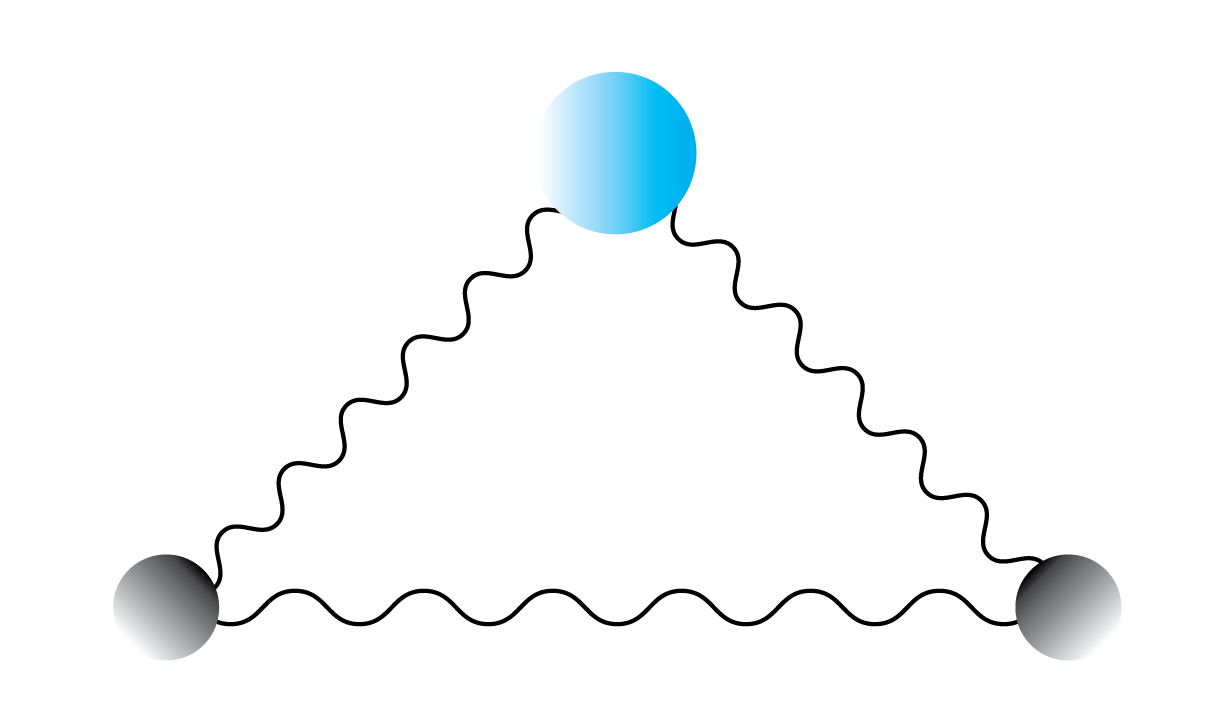
\includegraphics[scale=0.7]{figures/methods/harmonic-oscillator_polyatomic.png}
    \caption{Triatomic molecule (H$_2$O) ball-spring representation. The blue and grey circle represents oxygen and hydrogen, respectively.}
    \label{fig:oscillator:water}
\end{figure}

In polyatomic molecules, each vibrational mode can be approximated to a normal vibrational mode. With an analogous approximation from diatomic, the vibrational term value $G(v_i)$ associated with each normal vibration $i$, is given by:
\[G(v_i) = \omega_i \enclose{v_i + \frac{d_i}{2}}\]

where $d_i$ represents the degree of degeneracy.\\

\subsubsection{Selection rules}
\label{sec:mol-vibration:selection-rule}

When two vibrational states undergo absorption or emission transitions, there is usually an interaction between the molecule and the electric component of electromagnetic radiation. Therefore, the electric dipole moment ($\vec{\mu}$) determines the selection rule for vibrational transitions in the infrared spectrum.

The vibrational transition intensity is proportional to $|R_v|^2$, the square of the vibrational transition moment $R_v$, defined by:

\begin{equation}
    \label{eqn:vib:selctrion-rule}
    R_v = \int \psi^{'} \vec{\mu} \psi{''} d\tau_v
\end{equation}

where $\psi{''}$ and $\psi{'}$ are initial and final vibrational wavefunctions, respectively.\\

A transition is only allowed if the transition dipole integral is non-zero, i.e.:

\begin{align*}
    \begin{split}
        R_v &= 0 \text{ forbidden transition} \\
        R_v &\neq 0 \text{ allowed transition}
    \end{split}
\end{align*}
For diatomic molecules, within the harmonic approximation, $R_v$ is non-zero only when $\Delta v = \pm 1$. Anharmonicity can lead to $\Delta v = \pm 2, \pm 3, ...$, overtone transitions but they are generally weak.

In general, there are simple requirements for the integral of Eq. \ref{eqn:vib:selctrion-rule} to be non-zero; they are as follows.

When both $\psi{''}$ and $\psi{'}$ are non-degenerate, the symmetry species of the quantity to be integrated should be totally symmetric; that is:

\[\Gamma(\psi^{'}) \otimes \Gamma(\vec{\mu}) \otimes \Gamma(\psi^{''}) = A\]

where $A$ denotes the totally symmetric species of any non-degenerate point group, and $\Gamma$ stands for symmetry representation.

For degenerate states:
\[\Gamma(\psi^{'}) \otimes \Gamma(\vec{\mu}) \otimes \Gamma(\psi^{''}) \supset A\]

A brief overview of molecular vibration for diatomic and polyatomic molecules has been discussed, along with the selection rule for observing IR active vibrational transition modes using quantum mechanics. The following section deals with the quantum mechanical theory of molecular rotation.
